% compile with
%   pdflatex --shel-escape p03-matrizes
% or
%   latexmk -pvc -pdf -latexoption=--shell-escape p03-matrizes
%

\documentclass[11pt]{practice}

\begin{document}

\institution{UFOP\quad DECOM}
\course{Programação de Computadores I}
\subtitle{Aula prática 2}
\title{Vetores e Matrizes}
% \author{José Romildo Malaquias\thanks{\url{romildo@iceb.ufop.br}}}
\date{2013--2}
\maketitle

\begin{abstract}
  Nesta aula será explorada a noção de vetores para desenhar gráficos de
  funções.
\end{abstract}

\tableofcontents


\section{Desenho de gráficos}

Para desenhar um gráfico de uma maneira simples, siga os passos seguintes:
\begin{enumerate}
  \item É bom limpar a janela de gráficos (também chamada janela de
  figuras) antes de começar a construir um novo desenho. Para tanto use
  o comando \texttt{clf}.

  \item Defina um vetor\footnote{Vetores são matrizes
    unidimensionais. Um vetor linha é uma matriz contendo somente uma
    linha. Um vetor coluna é uma matriz contendo somente uma coluna}
  contendo as abscissas dos pontos a serem plotados. A notação de
  progressão aritmética pode ser usada, indicando o limite inferior, a
  razão, e o limite superior.

  Exemplo:
  \begin{lst}{scilab}
// vetor linha formado pelos valores das
// abscissas dos pontos a serem plotados

// limite inferior: -pi
// razão (ou passo): 0.2
// limite superior: pi

x = [-%pi : 0.2 : %pi];
  \end{lst}

  \item Defina outro vetor linha contendo as ordenadas dos pontos a
  serem plotados. Pode-se usar operações aritméticas ou funções com
  vetores para construir este vetor a partir do vetor das abscissas.

  Para realizar uma operação entre um escalar $k$ e cada elemento de uma
  matriz $A$, produzindo a matriz dos resultados, temos:
  \begin{center}
    \begin{tabular}{p{2cm}l} \hline
      \textbf{operação} & \textbf{descrição} \\\hline
      \texttt{$k$ + $A$}\newline \texttt{$A$ + $k$}  & adição \\\hline
      \texttt{$k$ - $A$}\newline \texttt{$A$ - $k$}  & subtração \\\hline
      \texttt{$k$ * $A$}\newline \texttt{$A$ * $k$}  & multiplicação \\\hline
      \texttt{$A$ / $k$}\newline \texttt{$k$ ./ $A$}  & divisão \\\hline
      \texttt{$A$ .\textasciicircum\ $k$}  & potenciação \\\hline
    \end{tabular}
  \end{center}

  Para realizar uma operação com duas matrizes $A$ e $B$ entre os
  elementos correspondentes, produzindo a matriz dos resultados, temos:
  \begin{center}
    \begin{tabular}{ll} \hline
      \textbf{operação} & \textbf{descrição} \\\hline
      \texttt{$A$ + $B$} & adição \\\hline
      \texttt{$A$ - $B$} & subtração \\\hline
      \texttt{$A$ .* $B$} & multiplicação \\\hline
      \texttt{$A$ ./ $B$} & divisão \\\hline
      \texttt{$A$ .\textasciicircum\ $B$} & potenciação \\\hline
    \end{tabular}
  \end{center}

  Várias funções podem ser aplicadas a matrizes, e a função será
  realizada individualmente com cada elemento da matriz, produzindo a
  matriz dos resultados.

  Exemplo:
  \begin{lst}{scilab}
// vetor linha formado pela aplicação da função
// f(x) = x * sin(x) - x^3 / (2*pi)
// a cada elemento do vetor das abscissas

y = x .* sin(x) - x .^ 3 / (2*%pi);
  \end{lst}

  \item Para desenhar o gráfico, use a função \texttt{plot}, passando o
  vetor das abscissas e o vetor das ordenadas como argumentos. Pode-se
  desenhar vários gráficos ao mesmo tempo. Para cada gráfico use dois
  vetores (abscissas e ordenadas).

  A função \texttt{title} permite dar um título ao desenho.

  As funções \texttt{xlabel} e \texttt{ylabel} podem ser usadas para
  rotular os eixos do desenho.

  A função \texttt{legend} coloca legendas nos gráficos desenhados.

  A expressão \texttt{set(gca(), "grid", [1 1])} desenha uma grade.

  Exemplo:
  \begin{lst}{scilab}
// desenha o gráfico
plot(x, y);
title("Gráfico de funções");
xlabel("x");
ylabel("y");
legend("Resultado");
set(gca(), "grid", [1 1]);
  \end{lst}
  A seguir temos o desenho produzido por este exemplo.
  \begin{center}
    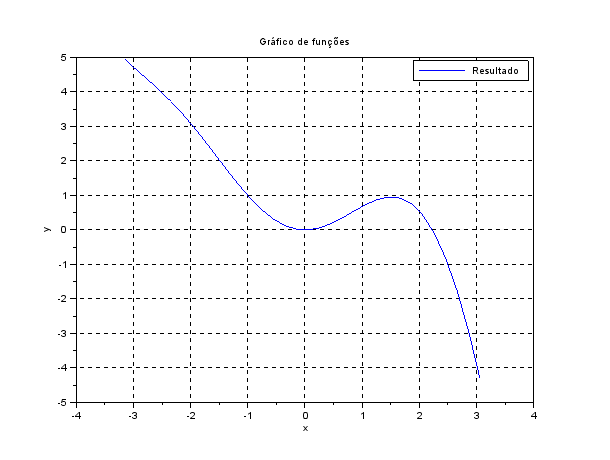
\includegraphics[width=\linewidth]{images/grafico}
  \end{center}
\end{enumerate}

\begin{task}[breakable]{Posição e velocidade de uma bola \numex{2.10}}{}
  Se uma bola estacionária é lançada da altura $h_0$ acima da superfície
  da Terra, com velocidade vertical $v_0$, a posição e a velocidade da
  bola como função do tempo serão dadas pelas equações
  \[ h(t) = \frac{1}{2}gt^2 + v_0t + h_0 \]
  \[ v(t) = gt + v_0 \] onde $g$ é a aceleração da gravidade
  ($-9,8m/s^2$), $h$ é a altura acima da superfície da Terra (assumindo
  ausência de atrito do ar) e $v$ é a componente vertical da velocidade.

  Escreva um programa que solicite ao usuário a altura inicial da bola
  em $m$ e a velocidade de lançamento da bola em $m/s$, depois desenhe a
  altura e velocidade em função do tempo. Não deixe de incluir as
  legendas apropriadas no seu desenho.

  \begin{runexample}
Lançamento de uma bola
----------------------
altura inicial da bola (m): 20
velociade de lançamento da bola (m/s): 46
  \end{runexample}
  \begin{center}
    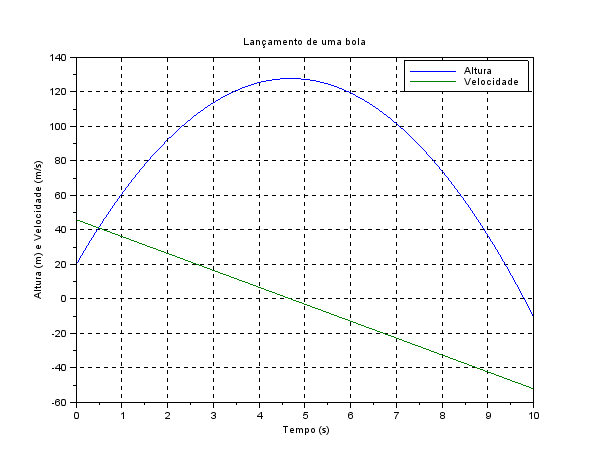
\includegraphics[width=\linewidth]{images/bola}
  \end{center}

  \tcblower
  \solution
  \lstinput{scilab}{listings/p03/bola.sce}
  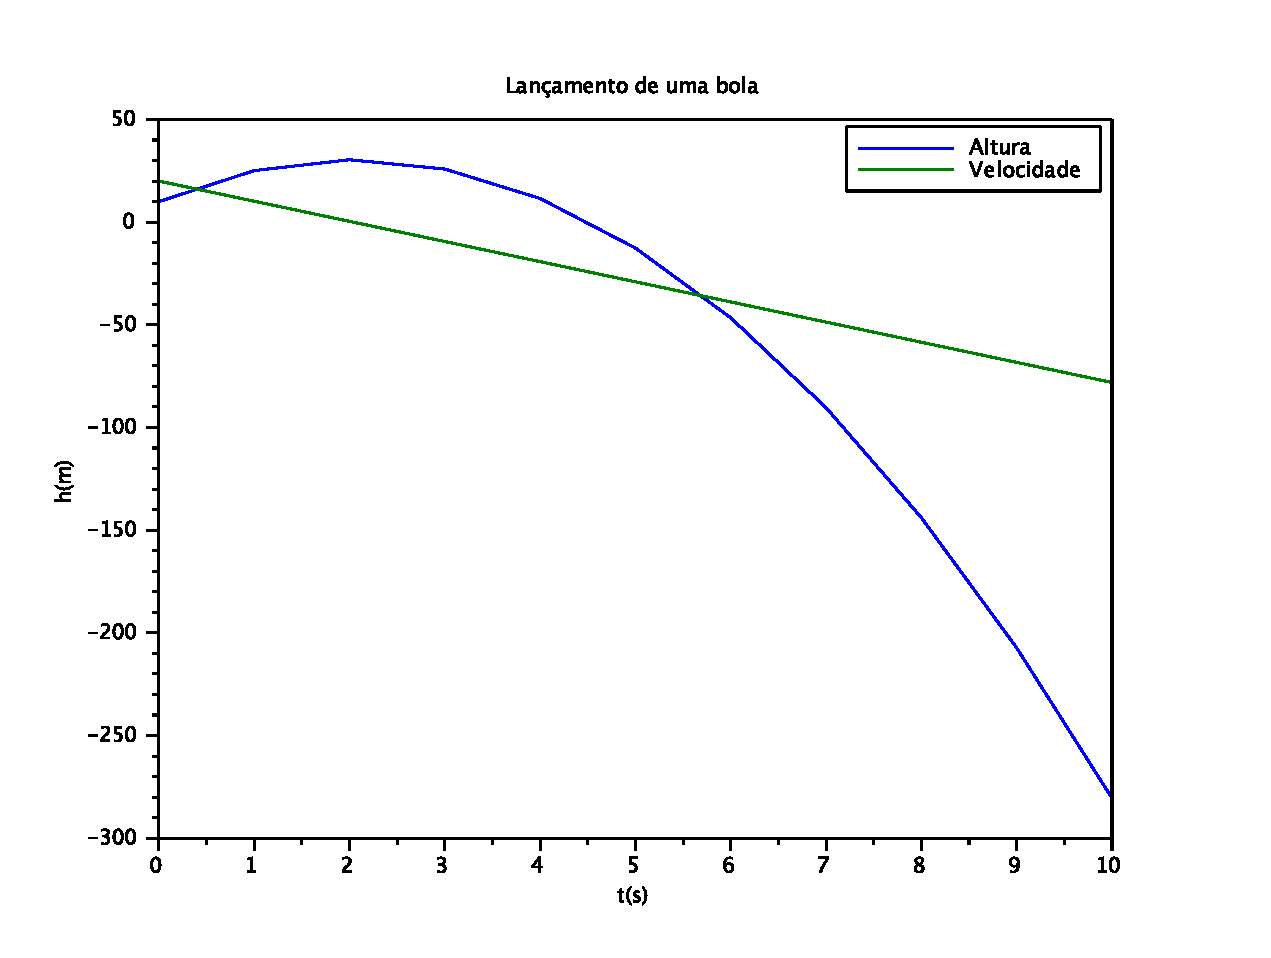
\includegraphics[width=\linewidth]{listings/p03/bola.pdf}
\end{task}

\end{document}
